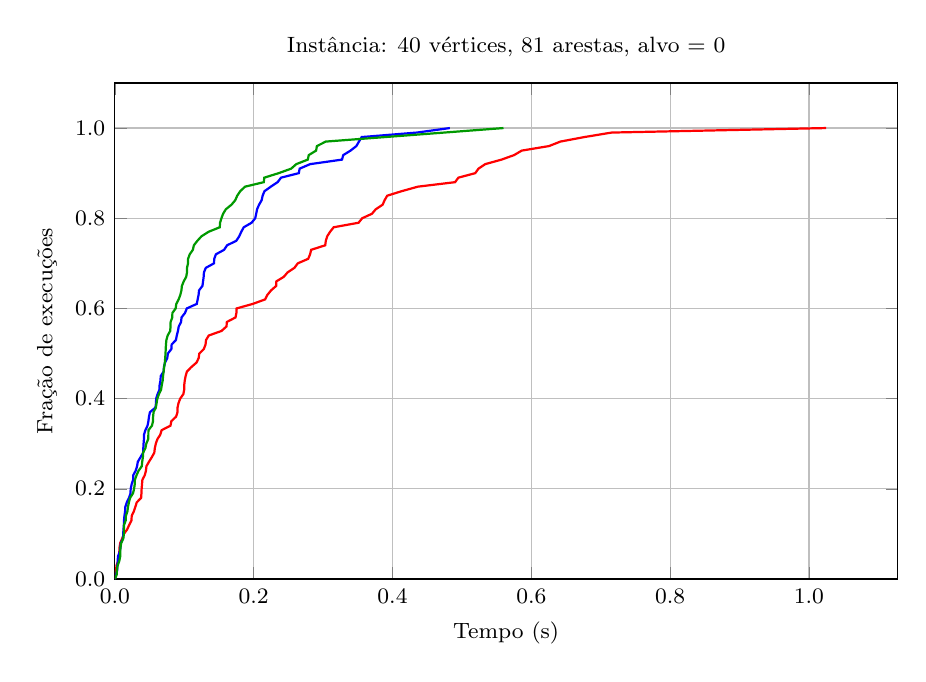
\begin{tikzpicture}
    \begin{axis}
    [
    width=0.95\textwidth,
    height=0.65\textwidth,
    xlabel={\footnotesize Tempo (s)},
    ylabel={\footnotesize Fração de execuções},
    title={\footnotesize Instância: 40 vértices, 81 arestas, alvo = 0},
    ymin=0,
    xmin=0,
    xtick={0.0,0.2,0.4,0.6,0.8,1.0},
    xticklabels={
            \footnotesize 0.0,
            \footnotesize 0.2,
            \footnotesize 0.4,
            \footnotesize 0.6,
            \footnotesize 0.8,
            \footnotesize 1.0},
    ytick={0.0,0.2,0.4,0.6,0.8,1.0},
    yticklabels={
            \footnotesize 0.0,
            \footnotesize 0.2,
            \footnotesize 0.4,
            \footnotesize 0.6,
            \footnotesize 0.8,
            \footnotesize 1.0},
    legend pos=south east,
    grid=major,
    legend to name=legendaMetodos, % salva a legenda
    legend columns=3,
    legend style={/tikz/every even column/.append style={column sep=1cm}}
]

% Linha vermelha - Mult Start (N=100 execuções)
\addplot+[
    mark=none,
    thick,
    red,
] coordinates {
    (0,0) (0.000632,0.01) (0.00181,0.02) (0.002331,0.03) (0.004736,0.04) (0.005643,0.05) (0.006406,0.06) (0.006724,0.07) (0.007706,0.08) (0.010621,0.09) (0.013021,0.1) (0.017736,0.11) (0.020646,0.12) (0.023954,0.13) (0.024236,0.14) (0.027313,0.15) (0.029496,0.16) (0.031547,0.17) (0.037815,0.18) (0.038277,0.19) (0.038553,0.2) (0.039101,0.21) (0.039656,0.22) (0.043027,0.23) (0.044767,0.24) (0.045467,0.25) (0.049114,0.26) (0.053158,0.27) (0.056794,0.28) (0.057544,0.29) (0.058977,0.3) (0.061211,0.31) (0.065408,0.32) (0.067346,0.33) (0.0801,0.34) (0.081401,0.35) (0.088155,0.36) (0.090264,0.37) (0.09028,0.38) (0.091681,0.39) (0.094101,0.4) (0.098676,0.41) (0.099907,0.42) (0.099922,0.43) (0.100684,0.44) (0.101936,0.45) (0.103795,0.46) (0.1102,0.47) (0.117659,0.48) (0.120744,0.49) (0.121632,0.5) (0.128157,0.51) (0.130645,0.52) (0.131343,0.53) (0.135287,0.54) (0.153573,0.55) (0.160806,0.56) (0.161366,0.57) (0.173776,0.58) (0.175115,0.59) (0.175372,0.6) (0.198607,0.61) (0.216443,0.62) (0.219741,0.63) (0.225004,0.64) (0.232487,0.65) (0.232657,0.66) (0.243291,0.67) (0.24891,0.68) (0.258715,0.69) (0.26353,0.7) (0.278519,0.71) (0.281222,0.72) (0.282823,0.73) (0.303047,0.74) (0.303923,0.75) (0.305949,0.76) (0.310113,0.77) (0.315213,0.78) (0.35106,0.79) (0.356332,0.8) (0.37048,0.81) (0.37592,0.82) (0.385782,0.83) (0.388632,0.84) (0.392375,0.85) (0.413208,0.86) (0.436497,0.87) (0.490144,0.88) (0.494925,0.89) (0.519258,0.9) (0.523873,0.91) (0.533659,0.92) (0.557047,0.93) (0.575165,0.94) (0.586183,0.95) (0.625416,0.96) (0.6419,0.97) (0.676312,0.98) (0.715766,0.99) (1.02488,1.0)
};
\addlegendentry{\footnotesize MULTI-START}

% Linha azul - GRASP_FIXO (N=100 execuções)
\addplot+[
    mark=none,
    thick,
    blue,
] coordinates {
    (0,0) (0.001834,0.01) (0.003413,0.02) (0.003629,0.03) (0.00415,0.04) (0.004412,0.05) (0.007022,0.06) (0.007975,0.07) (0.0087,0.08) (0.011698,0.09) (0.01203,0.1) (0.012376,0.11) (0.012958,0.12) (0.01316,0.13) (0.013761,0.14) (0.014708,0.15) (0.015065,0.16) (0.017188,0.17) (0.020347,0.18) (0.022473,0.19) (0.022772,0.2) (0.024155,0.21) (0.026271,0.22) (0.026405,0.23) (0.029907,0.24) (0.031963,0.25) (0.033053,0.26) (0.03692,0.27) (0.040755,0.28) (0.040976,0.29) (0.041333,0.3) (0.041859,0.31) (0.041944,0.32) (0.043949,0.33) (0.047048,0.34) (0.048295,0.35) (0.049148,0.36) (0.05053,0.37) (0.058357,0.38) (0.059303,0.39) (0.059468,0.4) (0.061536,0.41) (0.064294,0.42) (0.06445,0.43) (0.065682,0.44) (0.066048,0.45) (0.070253,0.46) (0.070667,0.47) (0.072294,0.48) (0.075498,0.49) (0.07635,0.5) (0.081435,0.51) (0.081785,0.52) (0.087967,0.53) (0.089238,0.54) (0.090885,0.55) (0.092048,0.56) (0.095351,0.57) (0.096038,0.58) (0.101064,0.59) (0.103583,0.6) (0.117967,0.61) (0.119292,0.62) (0.120611,0.63) (0.121279,0.64) (0.126164,0.65) (0.127061,0.66) (0.127889,0.67) (0.12834,0.68) (0.131015,0.69) (0.142832,0.7) (0.143148,0.71) (0.145576,0.72) (0.157374,0.73) (0.161647,0.74) (0.174943,0.75) (0.179176,0.76) (0.182134,0.77) (0.18569,0.78) (0.196958,0.79) (0.202207,0.8) (0.203656,0.81) (0.204899,0.82) (0.207748,0.83) (0.211467,0.84) (0.212869,0.85) (0.215562,0.86) (0.224717,0.87) (0.234477,0.88) (0.239409,0.89) (0.265007,0.9) (0.26622,0.91) (0.281357,0.92) (0.327259,0.93) (0.329013,0.94) (0.339574,0.95) (0.347873,0.96) (0.351706,0.97) (0.355585,0.98) (0.435194,0.99) (0.482585,1.0)
};
\addlegendentry{\footnotesize GRASP-FIXO}

% Linha verde - GRASP_REATIVO (N=100 execuções)
\addplot+[
    mark=none,
    thick,
    green!60!black,
] coordinates {
    (0,0) (0.002713,0.01) (0.00286,0.02) (0.004043,0.03) (0.006405,0.04) (0.007703,0.05) (0.007761,0.06) (0.008052,0.07) (0.009182,0.08) (0.012158,0.09) (0.012949,0.1) (0.012971,0.11) (0.013276,0.12) (0.015629,0.13) (0.015858,0.14) (0.018092,0.15) (0.018886,0.16) (0.020239,0.17) (0.021942,0.18) (0.026126,0.19) (0.027664,0.2) (0.028625,0.21) (0.028834,0.22) (0.031181,0.23) (0.034108,0.24) (0.038723,0.25) (0.039354,0.26) (0.040339,0.27) (0.04066,0.28) (0.043965,0.29) (0.045218,0.3) (0.047969,0.31) (0.048268,0.32) (0.048305,0.33) (0.053441,0.34) (0.054925,0.35) (0.0551,0.36) (0.055721,0.37) (0.058997,0.38) (0.060107,0.39) (0.061206,0.4) (0.063514,0.41) (0.066584,0.42) (0.067585,0.43) (0.068903,0.44) (0.069387,0.45) (0.070213,0.46) (0.071002,0.47) (0.072006,0.48) (0.072488,0.49) (0.072979,0.5) (0.073244,0.51) (0.073601,0.52) (0.074246,0.53) (0.076044,0.54) (0.079686,0.55) (0.080191,0.56) (0.08031,0.57) (0.082714,0.58) (0.082867,0.59) (0.087573,0.6) (0.088473,0.61) (0.091859,0.62) (0.094287,0.63) (0.095868,0.64) (0.09657,0.65) (0.099191,0.66) (0.102741,0.67) (0.103927,0.68) (0.103936,0.69) (0.105378,0.7) (0.105471,0.71) (0.107861,0.72) (0.112348,0.73) (0.11383,0.74) (0.118859,0.75) (0.124825,0.76) (0.135069,0.77) (0.15112,0.78) (0.15156,0.79) (0.153516,0.8) (0.155957,0.81) (0.15994,0.82) (0.168003,0.83) (0.173467,0.84) (0.176268,0.85) (0.180609,0.86) (0.187561,0.87) (0.214536,0.88) (0.215297,0.89) (0.236042,0.9) (0.254049,0.91) (0.261351,0.92) (0.277943,0.93) (0.279339,0.94) (0.289929,0.95) (0.291039,0.96) (0.303858,0.97) (0.55991,1.0)
};\addlegendentry{\footnotesize GRASP-REATIVO}
    \end{axis}
    \end{tikzpicture}